% Ideia desse capitulo: Apresentar o desenvolvimento do projeto-
% 
% Deficiências do projeto atual
% Propostas de melhorias
% 
% Documentação do Projeto
% Adaptação do servidor python
% Implementação do cliente Android
% Adaptação do cliente Python


\chapter{Descrição e desenvolvimento do projeto}


    Neste capítulo são apresentados o desenvolvimento da proposta do projeto e também sua implementação no FlexA. Inicialmente serão abordados as deficiências encontradas no projeto atual e a motivação para corrigi-las. Então será apresentada a documentação desenvolvida para que o projeto possa ser viável a longo prazo, e em outra sessão será detalhado as adaptações realizadas no módulo servidor para que esse passasse a ser compatível com a nova especificação. Com o novo servidor pronto, será apresentado a implementação do cliente para Android e por fim, em outra sessão será mostrado a adaptação do cliente atual em Python para a nova especificação do servidor.

    \section{Deficiências da versão atual do FlexA}
    \section{Documentação de todo o projeto}
    \section{Adaptação do servidor em Python}
    \section{Implementação do cliente Android}
    \section{Adaptação do cliente em Python}
    
    
    %
    %
    % Distribuir e organizar o texto já escrito nessas sessões.
    %
    %
    
    

        A versão atual do FlexA não possuí um modelo de programação bem definido, com pouca documentação e a inexistência de uma convenção do fluxo de dados dentro do sistema. Carente também de uma padronização explicita da transmissão dos metadados.
        
        Dessa forma um estudo mais a fundo do sistema foi realizado, utilizando a pouca documentação que existia do sistema e a análise de todo o código-fonte, para entender o real funcionamento e comportamento do sistema, e como era definida a estrutura atual do projeto. Após esse estudo foi criado um diagrama para representar o estado atual dos módulos do sistema, e suas dependências conforme pode ser visto na Figura \ref{fig:pacotesMario}.
        
        \begin{figure}[!ht]
            \centering
            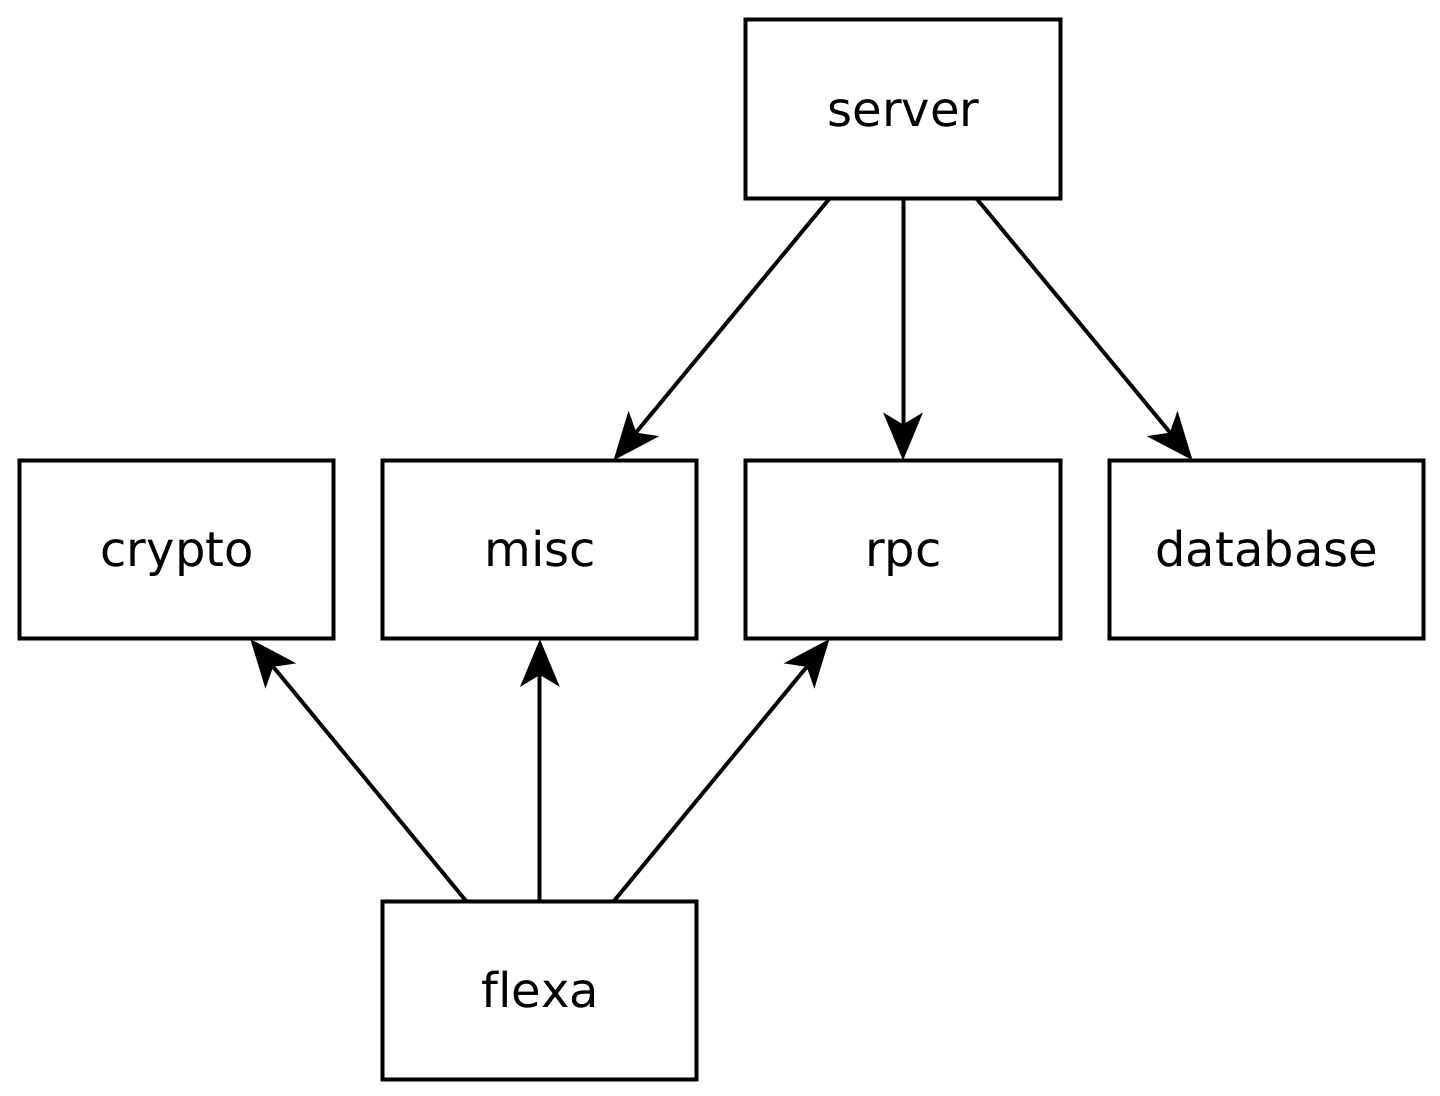
\includegraphics[width=10cm]{pacotesMario.png}
            \caption{Módulos do sistema atual e suas dependências. ~\cite{mario}.}
            \label{fig:pacotesMario}
        \end{figure}
        
        Esse diagrama foi gerado a partir do estudo do código-fonte da versão atual do projeto. Apenas por esse diagrama já é possível notar que o módulo Servidor em momento algum utiliza os serviços de criptografia, e que apenas o servidor tem acesso aos bancos de dados de metadados.
        
        Além do diagrama de módulos do sistema também foi criado um diagrama de classes, para que fosse possível analisar a estrutura mais interna dos módulos. Esse diagrama é apresentado na figura \ref{fig:classesMario}. Embora seja um diagrama de classes, alguns abusos de notação tiveram que ser utilizados devido a lacuna existente entre a representação dos diagramas de Classes da Unified Language Model (UML)~\cite{umlClasses} e a linguagem Python em que o FlexA é desenvolvido.
        
        \begin{figure}[!ht]
        \centering
        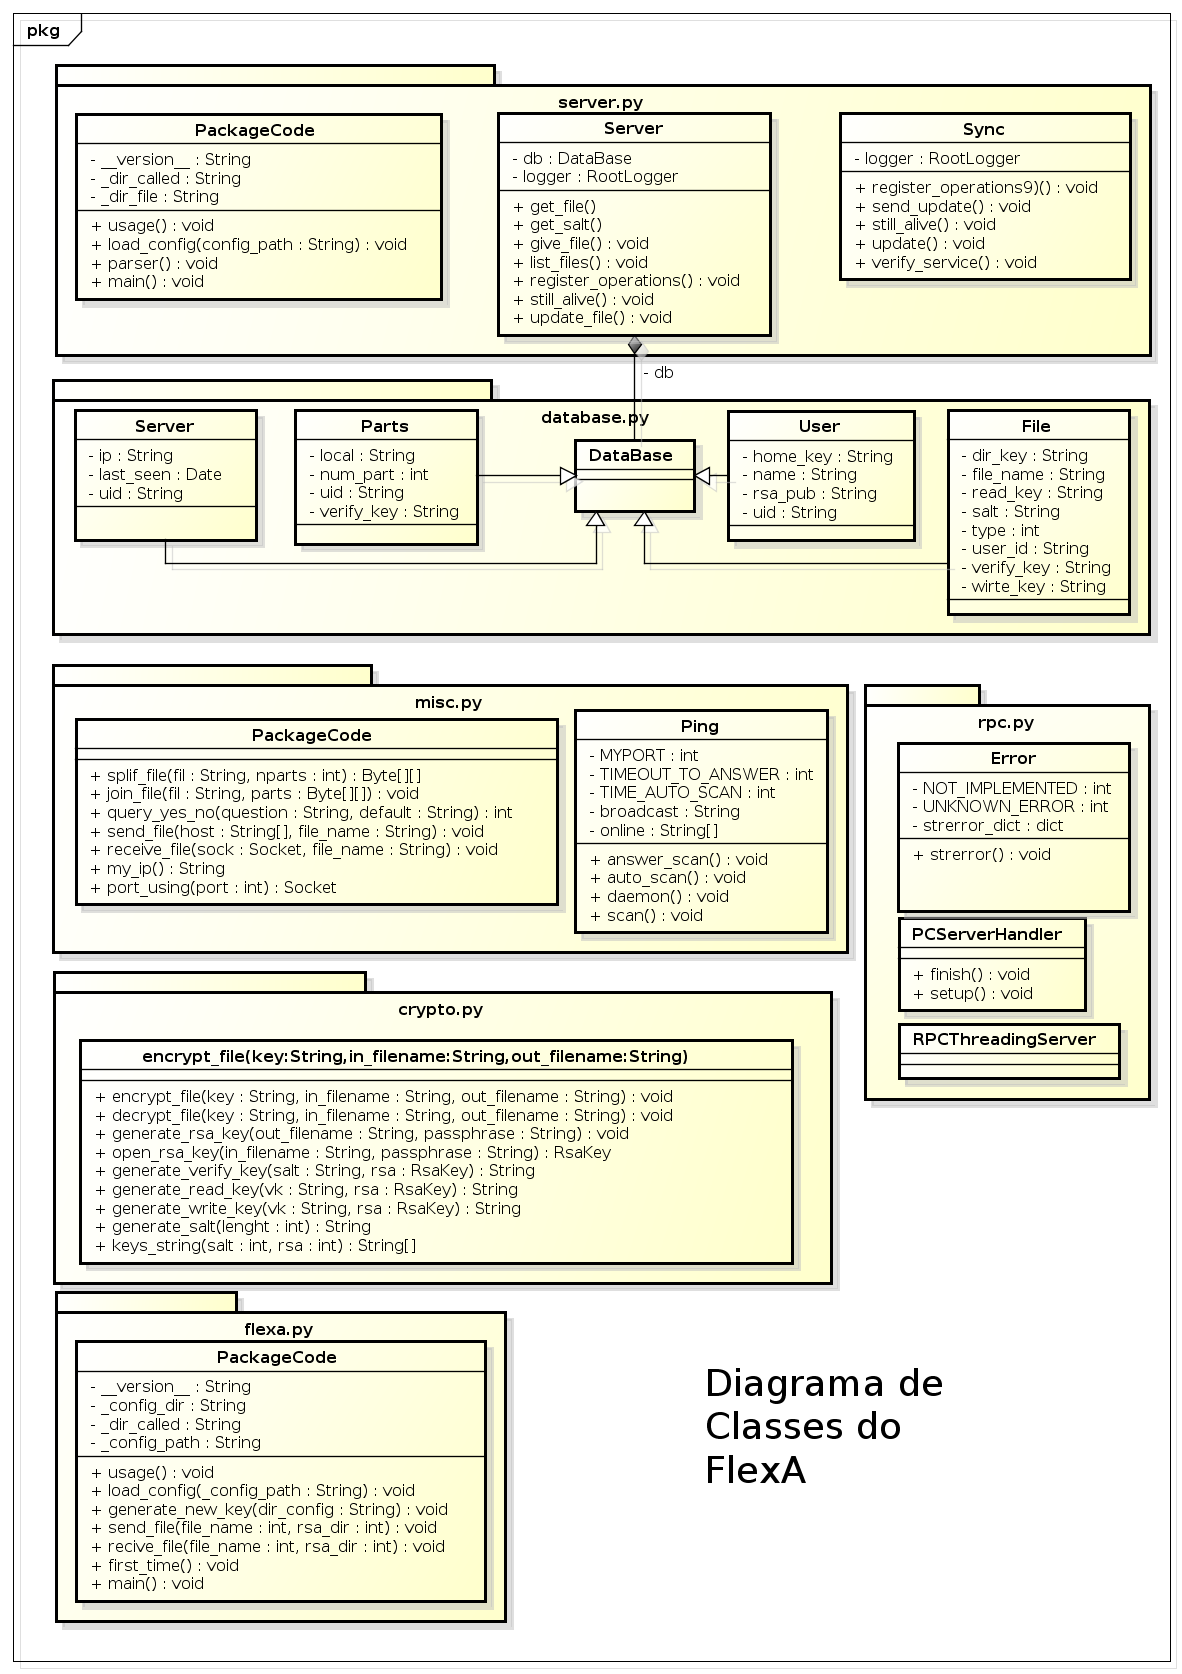
\includegraphics[width=14cm]{classesMario.png}
        \caption{Classes e pacotes (arquivos) que estruturam a versão atual do FlexA}
        \label{fig:classesMario}
        \end{figure}
             

        Analisando o diagrama de classes apresentado na Figura \ref{fig:classesMario} é possível perceber que muitas atividades diferentes e classes distintas pertencem a um mesmo pacote. Até esse trabalho, como todo o FlexA era desenvolvido apenas em Python, não havia problema em manter o padrão de desenvolvimento atual. 
        
        Conforme a proposta desse trabalho, desenvolver um cliente para Android do FlexA e melhorar os quesitos de abertura do FlexA, se mostrou necessário realizar alterações no projeto para que fosse possível a execução desses objetivos.
        
        Em um primeiro momento foi feito o levantamento dos requisitos do FlexA, junto com os objetivos de melhoria do código existente. Dessa forma foi elaborado o seguinte diagrama UML de casos de uso de acordo com ~\cite{umlCasosDeUso}. O diagrama com os casos de uso é apresentado na Figura \ref{fig:casosDeUsoGabriel}.
        
        \begin{figure}[!ht]
        \centering
        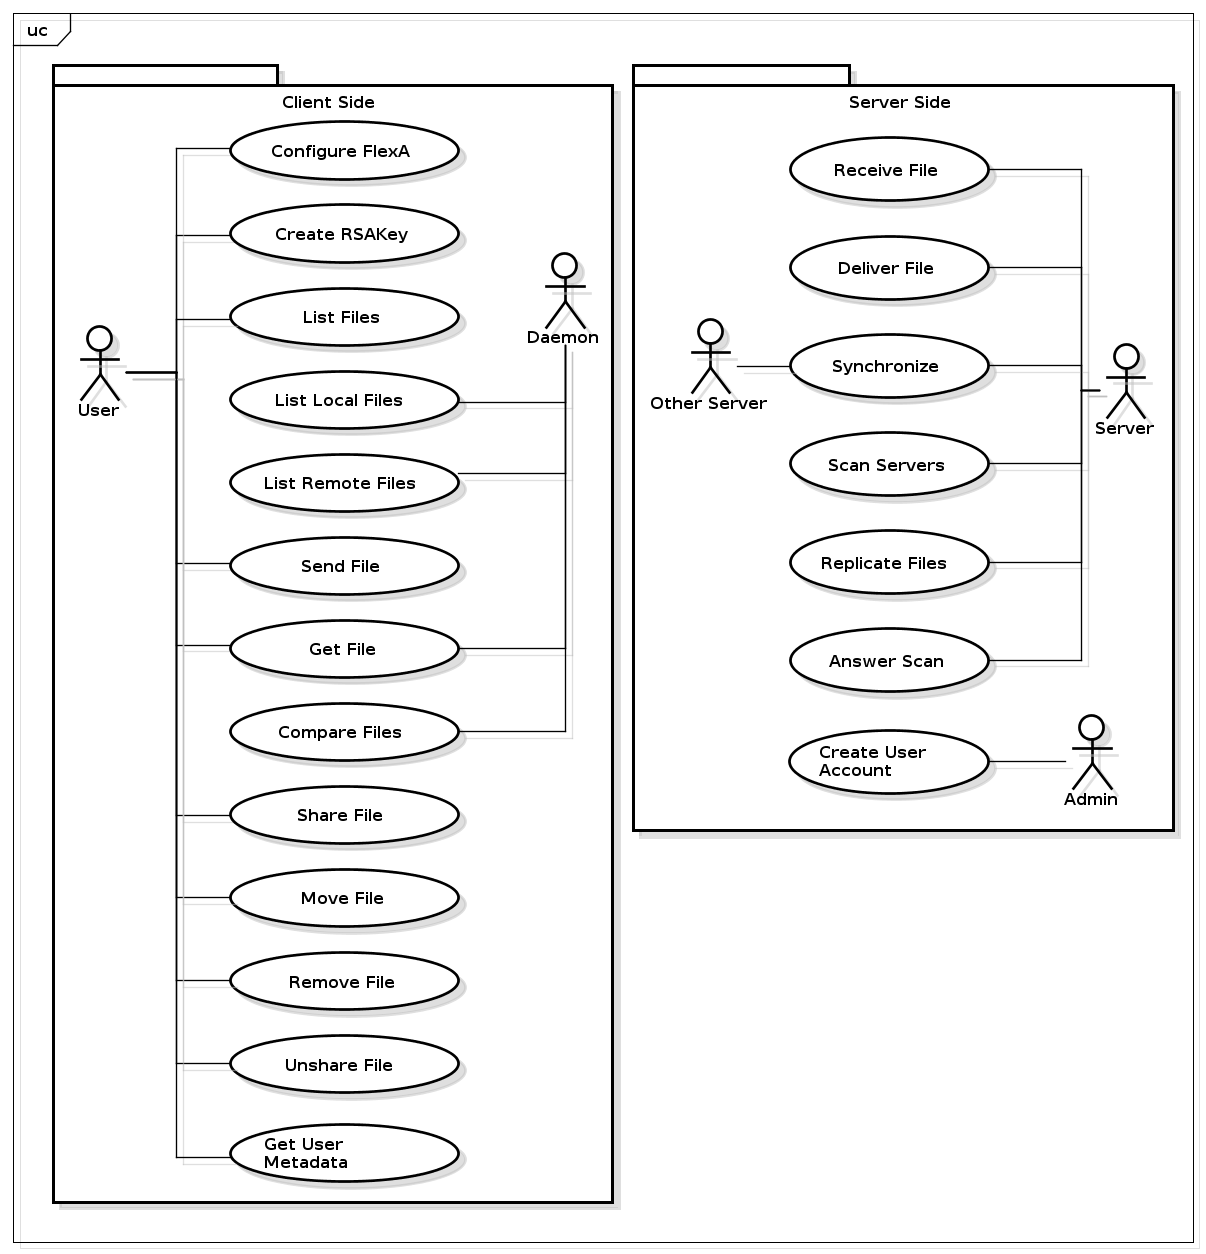
\includegraphics[width=15cm]{casosDeUsoGabriel.png}
        \caption{Diagrama de Casos de uso com os requisitos funcionais do FlexA.}
        \label{fig:casosDeUsoGabriel}
        \end{figure}
    
        Uma vez definidas quais são as funcionalidades que são esperadas do sistema, iniciou-se uma analise mais profunda das comunicações entre cliente e servidor. Poucas informações foram encontradas em ~\cite{mario} e ~\cite{silas} sobre a padronização da comunicação entre cliente e servidores, e o pouco que foi encontrado já estava defasado devido a grandes alterações no sistema desde então. Dessa forma foi necessário analisar o código fonte e entender exatamente como eram feitas as comunicações nas diversas operações existem.
        
        Após o estudo da comunicação entre cliente e servidor ~\cite{mario} formalizou-se, utilizando a notação para protocolos de comunicação apresentada em ~\cite{ross} que é mostrada na tabela \ref{tab:notacao}.
        
        \begin{table}
        
        \centering
        \begin{tabular}{|l|l|}
        \hline
        
        $C$ & módulo cliente ou usuário \\
        \hline
        $S$ & módulo servidor \\
        \hline
        $privKey_{X}$ & chave privada $X$ \\
        \hline
        $pubKey_{X}$ & chave pública $X$ correspondente a $privKey_{X}$\\
        \hline
        $C \rightarrow S : dado$ & $C$ envia $dado$ para $S$\\
        \hline
        $C \rightarrow S : {dado}_{pubKey_{x}}$ & $C$ envia $dado$ criptografado com a chave pública $X$ para $S$\\
        \hline

        \end{tabular}
        \caption{Notação utilizada para definição de protocolos de comunicação ~\cite{ross}.}
        \label{tab:notacao}
        \end{table}
        
        
        
        Formalizadas as definições que serão utilizadas a seguir, são apresentados os protocolos para as comunicações. Esses protocolos foram elaborados baseados no código fonte ~\cite{mario} já inserindo as adaptações para fornecer maior modularização, compatibilidade e segurança ao sistema.
        

        A primeira formalização é o protocolo para solicitação dos metadados do usuário que acaba de iniciar o FlexA pela primeira vez ou quando seja necessário obter seu \textit{userID}. Isso é feito com base em sua chave pública previamente cadastrada no sistema por um administrador. O protocolo é apresentado na figura \ref{fig:protMetadadosUsuario}.
        
        \begin{figure}[!ht]
        
        \bordaProtocolo{
                $C \rightarrow S: pubKey_{C}$ \\
                $S \rightarrow C: \{userID, homeKey\}_{pubKey_{C}}$
        }
        
        \caption{Protocolo de requisição dos metadados de um usuário com base na sua chave pública.}
        \label{fig:protMetadadosUsuario}
        \end{figure}
        
        Com os metadados do usuário (\textit{userID} e \textit{homeKey} que é o identificador se sua pasta raiz) o usuário pode começar a utilizar o sistema enviando e recebendo arquivos.
        
        Para que o usuário possa enviar um arquivo para o sistema é necessário verificar se existe um arquivo com o mesmo nome no mesmo endereço especificado através do \textit{salt}. Caso o arquivo não exista ainda, é feito o cadastro e solicitado o \textit{salt} referente ao arquivo. Na figura \ref{fig:protGetSalt} é formalizado o protocolo de requisição do \textit{salt} de um arquivo. É importante ressaltar que \textit{fileName} é composto pelo nome completo do arquivo com o diretório em que o arquivo se encontra. Esse nome é relativo ao diretório mapeado do FlexA para o usuário, que é referenciado por \textit{userID}.

        \begin{figure}[!ht]
        \bordaProtocolo{
            $C \rightarrow S: fileName,userID$ \\
            $S \rightarrow C: salt$
        }
        \caption{Requisição do \textit{salt} de um arquivo}
        \label{fig:protGetSalt}
        \end{figure}
        
        Caso o \textit{salt} retornado pelo servidor seja igual $0$ é definido assumido que esse arquivo ainda não existe no servidor com esse nome.
        
        Já com o \textit{salt}, o módulo cliente gera o trio de chaves para o arquivo (VK, RK e WK), criptografa o arquivo utilizando a RK, faz a divisão do arquivo em $N$ porções caso necessário e envia cada porção para um servidor. Para enviar as porções aos servidores o módulo cliente faz primeiro o cadastro do arquivo no servidor e então envia as porções. Na figura \ref{fig:protSendFile} é descrito o protocolo para essa ação, onde $N$ é o número de porções em que o arquivo foi dividido, $directoryKey$ é o identificador do diretório que o arquivo está e $fileType$ é o tipo do arquivo (diretório ou arquivo comum).
        
        \begin{figure}[!ht]
        \bordaProtocolo{
            Para $i$ de $1$ até $N$: \\
            $C \rightarrow S_{i}: fileName,(VK,WK),directoryKey,userID,fileType$ \\
            $S_{i} \rightarrow C: port $
        }
        
        \caption{Cadastro do arquivo nos servidores e negociação da porta de envio do arquivo}
        \label{fig:protSendFile}
        \end{figure}
        
        Após o cadastro do arquivo e a negociação da porta de transmissão do arquivo, é feita a transmissão do arquivo em uma nova conexão com o servidor na porta $port$.
        
        Com a negociação pronta basta enviar para o servidor a porção correspondente. Essa comunicação é definida conforme o protocolo mostrado na figura \ref{fig:protSendFileData}.
        
        \begin{figure}[!ht]
        \bordaProtocolo{
            Para $i$ de $1$ até $N$: \\
            $C \rightarrow S_{i}: filePart_{i}$
        }
        \caption{Transmissão das porções dos arquivos aos servidores}
        \label{fig:protSendFileData}
        \end{figure}
        
        
        Com os protocolos já definidos é possível enviar um arquivo para o servidor. Mas ainda não é possível recupera-lo. A seguir serão tratados os protocolos envolvidos na recuperação dos arquivos enviados aos servidores.
        
        Para recuperar um arquivo, é de grande importância a capacidade de listar os arquivos de um diretório. Para essa ação é utilizado o protocolo da figura \ref{fig:protListFiles}.
        
        \begin{figure}[!ht]
        \bordaProtocolo{
            $C \rightarrow S: directoryKey$\\
            $S \rightarrow C: metaFile_{0}, metaFile_{1}, metaFile_{2},...,metaFile_{n}$
        }
        \caption{Requisição da lista dos arquivos em um diretório}
        \label{fig:protListFiles}
        \end{figure}
        
        Ao requisitar ao servidor os arquivos do diretório referenciado por $directoryKey$ o servidor manda pacotes de informação $metaFile$ referente aos arquivos. Cada pacote desse é composto por:
        \begin{itemize}
            \item nome do arquivo
            \item tamanho do arquivo
            \item dono do arquivo
            \item data de criação
            \item data de modificação
        \end{itemize}
        
        Essas características do arquivo são enviadas junto com o nome do arquivo para evitar acessos desnecessários ao servidor para recuperar cada uma dessas informações posteriormente. Isso influencia muito no tempo de resposta do sistema.
        
        Com a lista dos arquivos o usuário pode requisitar um arquivo especifico ao servidor. Ao requisitar o arquivo o módulo cliente faz a solicitação do \textit{salt} referente ao arquivo pelo atributo nome, com essa informação gera o trio de chaves do arquivo. Com o identificador do arquivo (\textit{verify key}) o cliente solicita a um servidor uma lista com quais servidores possuem as porções do arquivo. Essa comunicação é formalizada na figura \ref{fig:protWhoHasParts}.
        
         \begin{figure}[!ht]
        \bordaProtocolo{
            Requisição do Salt (Figura \ref{fig:protGetSalt}):\\
            $C \rightarrow S: fileName,userID $\\
            $S \rightarrow C: salt$\\
            
            Requisição dos servidores com as partes do arquivo:\\
            $C \rightarrow S: VK, userID$ \\
            $S \rightarrow C: (S_{0},1),(S_{0},2),(S_{1},1),(S_{1},3),(S_{2},2),(S_{2},3),...$
        }

        \caption{Requisição do salt de um arquivo, e posteriormente dos servidores que possuem as partes do arquivo}
        \label{fig:protWhoHasParts}
        \end{figure}
        
        Ao fazer a solicitação de quais servidores possuem as partes do arquivo desejado, o cliente recebe uma lista de registros de quais servidores possuem qual parte do arquivo, no seguinte formato: ($SERVIDOR$,$PARTE DO ARQUIVO$). Esse é o formato utilizado na figura \ref{fig:protWhoHasParts}.
        
        Com a lista dos servidores que possuem as partes do seu arquivo o cliente pode finalmente requisitar as partes do arquivo. Esse processo é feito de acordo com o protocolo apresentado pela figura \ref{fig:protGetPart}
        
        \begin{figure}[!ht]
        \bordaProtocolo{
            Para $i$ de $1$ até $N$:\\
                $S_{i} \rightarrow C: filePart_{i}$
        }
        \caption{Servidores enviando porções do arquivo para o cliente}
        \label{fig:protGetPart}
        \end{figure}
        
        Uma vez que o cliente tenha todas as partes do arquivo a junção dessas partes é feita e depois disso o arquivo é descriptografado utilizando a chave de criptografia \textit{read key}.
        
        A operação de atualização de um arquivo nos servidores é equivalente a remover o arquivo atual e cadastrar um novo arquivo. Como o protocolo de envio de arquivos já foi apresentado nas figuras \ref{fig:protSendFile} e \ref{fig:protSendFileData}, são feitas a seguir a definição da do protocolo de remoção de um arquivo dos servidores. Esse protocolo é apresentado na figura \ref{fig:protRemoveFile}.
        
        \begin{figure}[!ht]
        \bordaProtocolo{
            $C \rightarrow S: verifyKey,writeKey$
        }
        \caption{Protocolo que define a requisição para exclusão de um arquivo dos servidores}
        \label{fig:protRemoveFile}
        \end{figure}
        
        
        Como definido pelo protocolo de remoção de arquivos, o cliente envia ao servidor o arquivo que deseja excluir e a chave de escrita no arquivo. Então o servidor se encarrega de excluir o arquivo de sua base de dados e replicar a mensagem. A complexidade dessa tarefa fica oculta do lado do servidor liberando o cliente dessas tarefas, o que diminui o uso de banda e tempo de resposta para o cliente.
        
        Além de enviar, listar, excluir e atualizar os arquivos remotos uma operação que também é de grande importância é a de mover arquivos para outro diretório. No FlexA essa operação é feita totalmente no módulo servidor de forma que o cliente não necessita enviar novamente o arquivo ao move-lo de diretório. Essa operação tem o protocolo de comunicação especificado na figura \ref{fig:protMoveFile}.
        
        \begin{figure}[!ht]
        \bordaProtocolo{
            $ C \rightarrow S: verifyKey,writeKey,destinationFileName, directoryKey $
        }
        \caption{Protocolo para mover um arquivo.}
        \label{fig:protMoveFile}
        \end{figure}
        
        
        Outro recurso muito importante do FlexA é o compartilhamento de arquivos, que é implementado através do compartilhamento das chaves de criptografia. Para que seja possível fazer o compartilhamento e armazenar o estado deles o servidor cadastra esses dados criptografados utilizando a chave pública do usuário que recebe a autorização para acessar o arquivo compartilhado. O protocolo de comunicação para a execução desse procedimento é apresentado na figura \ref{fig:protShareFile}.
        
        \begin{figure}[!ht]
        \bordaProtocolo{
            $C \rightarrow S: verifyKey, pubKey_{B}, \{accessKeys\}_pubKey_{B}$
        }
        \caption{Protocolo para o compartilhamento de arquivos}
        \label{fig:protShareFile}
        \end{figure}
        
        Como mostrado na figura \ref{fig:protShareFile}, o cliente envia as chaves de acesso que desejar ao usuário $B$, cifrando-as com a chave pública de $B$. 
        
        Quando o usuário B desejar requisitar o arquivo que foi compartilhado com ele, o mesmo protocolo de recebimento de arquivos comuns, apenas omitindo a parte de solicitação do \textit{salt}, pois já possui as chaves de acesso ao arquivo. Para saber quais arquivos o usuário $B$ tem acesso ele deve listar os arquivos compartilhados cadastrados com sua chave pública, utilizando o protocolo exibido na figura \ref{fig:protListSharedFiles}.
        
        
     \begin{figure}[!ht]
        \bordaProtocolo{
        $C \rightarrow S: userID$
        }
        \caption{Protocolo para o listar os arquivos compartilhados com um usuário.}
        \label{fig:protListSharedFiles}
        \end{figure}
        
        Por fim, após compartilhar um arquivo, caso seja necessário remover o compartilhamento é necessário refazer a criptografia do arquivo, já que as chaves de acesso foram fornecidas a outro usuário no compartilhamento. Para remover o acesso a um arquivo compartilhado é utilizado o protocolo apresentado na figura \ref{fig:protRemoveShare}.
        
        \begin{figure}[!ht]
        \bordaProtocolo{
            $C \rightarrow S: verifyKey,pubKey_{B}$
        }
        \caption{Remove o acesso do usuário $B$ a um arquivo compartilhado pelo usuário $C$}
        \label{fig:protRemoveShare}
        \end{figure}
        
        
        Esses são todos os protocolos que coordenam a comunicação entre o módulo cliente e o servidor (e vice e versa). Com esses protocolos definidos e formalizados o sistema possui documentação suficiente para passar para a faze de implementação da versão Android do módulo cliente.
        
        
        \section{Módulo Cliente desenvolvido Android}
        
        
        Implementar o módulo cliente para dispositivos móveis que utilizem Android é uma tarefa bem mais complexa que a implementação para interface de linha de comando ou Command-line Interface (CLI) que existe atualmente, pois para se obter um resultado satisfatório é necessário o uso de tarefas assíncronas nas operações de entrada e saída, de modo a evitar o congelamento do aplicativo ao realizar essas tarefas ~\cite{androidAssyncTask}, além da complexidade de exibir as informações utilizando interface gráfica de usuário (GUI).
        
        Dessa forma o foco do desenvolvimento da versão Android do FlexA focou principalmente na conectividade e no uso dos padrões de desenvolvimento estabelecidos com a formalização dos protocolos de comunicação entre cliente e servidor. Como primeiro passo para nortear o desenvolvimento de módulos compatives com o FlexA foi a criação de uma interface de comunicação padrão que garante a compatibilidade entre módulos feitos em linguagens diferentes, desde que utilizado o XML-RPC para a comunicação. Essa interface de comunicação é apresentada na figura \ref{fig:interfaceComunicação}.
        
        \begin{figure}
        \centering
        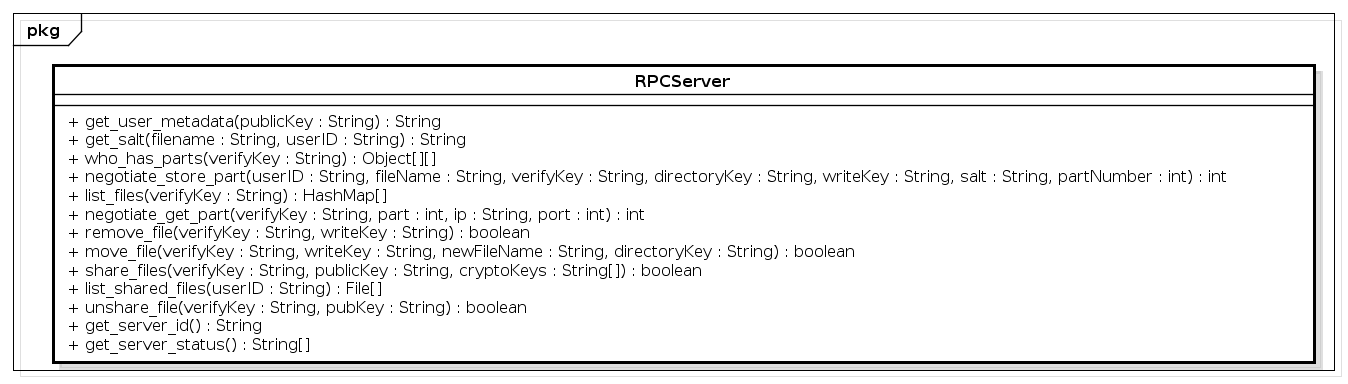
\includegraphics[width=14cm]{interfaceCom.png}
        \caption{Interface de comunicação dos servidores do FlexA.}
        \label{fig:interfaceComunicação}
        \end{figure}
        
        
        
        
        
        
           
        
        
        
        
        
        
        
        
        
        
        
        
        
        
        
        
        
        
        
        
        
        
        
        
        
        
        
        